\documentclass[main]{subfiles}

\begin{document}
\chapter*{Lecture 1: Finite length random walks on $\Z$} %Set chapter name
\addcontentsline{toc}{chapter}{Lecture 1} %Set chapter title
\setcounter{chapter}{1} %Set chapter counter
\setcounter{section}{0}

%The content goes here
\lecture{Siva Athreya}{Srivatsa B, Venkat Trivikram{$^\dagger$}}

\blfootnote{$^\dagger$ added illustrations}
\vspace{-0.75cm}
\section{Definitions}

Random walks serve as very useful models in many applications. They are simple to state and understand, yet they lead to lots of intractable questions.\\

\begin{notation}
    $ \N=\{k\in\Z:k\ge 1\} $ and $ \N_{0}=\N \cup \{0\} $\\
\end{notation}
We now proceed to construct what is called a ``simple random walk" on $ \Z $ of finite length $ N\in\N $.
The sample space $ \O_N $ and the event space $ \F_N $ are described below.
$$ \O_N:=\{(\o_1,\ldots,\o_N):\o_i\in\{-1,1\}\ \forall\ 1\le i\le N\} $$
$$ \F_N:=\{A:A\subseteq \O_N\} $$

The probability function $ \P_N:\O_N\to [0,1] $ is defined as
$$ \P_N(A):=\lvert A\rvert\ 2^{-N} $$

We also define random variables $ X_k $ and $ S_k $ on $ \O_N $ for $ 1\le k\le N $ as
$$ X_k:\O_N\to\{-1,1\}\lb X_k(\o):=\o_k$$
$$ S_k:\O_N\to\Z\lb S_k(\o):=\sum_{i=1}^kX_k(\o)\lb S_0(\o):=0 \text{ for all } \o\in\O_N$$
\begin{definition}
    Fix $ N\in\N $. The sequence of random variables $ \{S_k\}_{k=1}^N $ on $ (\O_N,\F_N, \P_N) $ is called a (symmetric) simple random walk on $\Z$, of finite length $ N $, starting at $ 0 $.
\end{definition}

\begin{figure}[H]
    \centering
    \caption{Three possible trajectories for $(S_{n})_{n=0}^{N}$}
    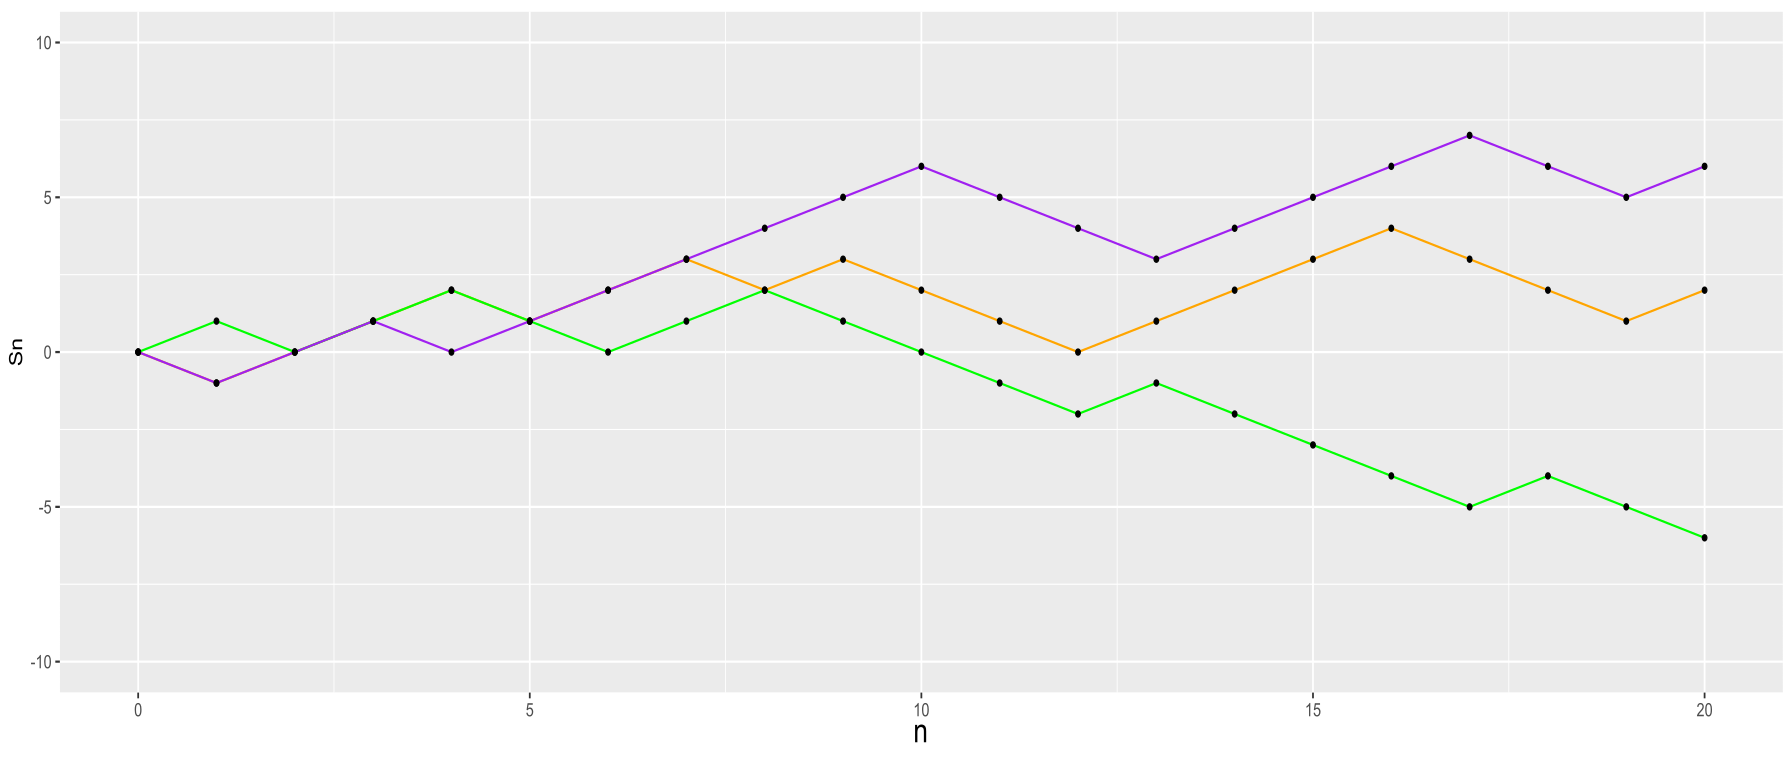
\includegraphics{threerw.png}
\end{figure}

In what follows, we suppress the subscript $ N $ while referring to the probability space $ (\O_N,\F_N, \P_N) $, and we assume that $ N\in\N $ is fixed.
%\newpage
\begin{obs}
    $\,$ \normalfont
    \begin{enumerate}
        \item[(a)] $\{X_k\}_{k=1}^N $ are iid, i.e. independent and identically distributed.
            \begin{proof}
                \begin{align*}
                    \P(X_k=1)=\P(\{\o\in\O:\o_k=1\}) & =2^{-N} |\{\o\in\O:\o_k=1\}| \\
                                                     & =2^{-N}2^{N-1}               \\
                                                     & =\frac{1}{2}                 \\
                                                     & =\P(X_k=-1)
                \end{align*}
                So $ \{X_k\}_{k=1}^N $ are identically distributed. Independence is left as an exercise.
            \end{proof}
            \item[(b)](Independent increments) For $ 1\le k_1\le k_2\le \ldots\le N $, $ \{S_{k_i}-S_{k_{i-1}}:1\le i\le N\} $ are independent random variables.

            \begin{proof}
                Observe that, for $ 1\le k<l\le N $, we have $ S_l-S_k=\sum_{i=k+1}^lX_i $. Therefore, if $ 1\le a<b\le c<d\le N $, we see that $ S_b-S_a $ and $ S_d-S_c $ are functions of disjoint sets of independent random variables, and hence the claim is true.
            \end{proof}

            \tikzset{every picture/.style={line width=0.5pt}} 
\begin{figure}[H]
	
	\centering
	\begin{tikzpicture}[x=0.75pt,y=0.75pt,yscale=-1,xscale=1]
		%uncomment if require: \path (0,268); %set diagram left start at 0, and has height of 268
		
		%Straight Lines [id:da20135057565865155] 
		\centering
		\draw    (85,23) -- (85,272) ;
		\draw [shift={(85,20)}, rotate = 90] [fill={rgb, 255:red, 0; green, 0; blue, 0 }  ][line width=0.08]  [draw opacity=0] (8.93,-4.29) -- (0,0) -- (8.93,4.29) -- cycle    ;
		%Straight Lines [id:da06573194358333212] 
		\draw    (56.8,190) -- (562.8,190) ;
		\draw [shift={(565.8,190)}, rotate = 180] [fill={rgb, 255:red, 0; green, 0; blue, 0 }  ][line width=0.08]  [draw opacity=0] (8.93,-4.29) -- (0,0) -- (8.93,4.29) -- cycle    ;
		%Straight Lines [id:da42483029683143725] 
		\draw    (85.3,190) -- (517.8,190) (139.3,187.5) -- (139.3,192.5)(193.3,187.5) -- (193.3,192.5)(247.3,187.5) -- (247.3,192.5)(301.3,187.5) -- (301.3,192.5)(355.3,187.5) -- (355.3,192.5)(409.3,187.5) -- (409.3,192.5)(463.3,187.5) -- (463.3,192.5)(517.3,187.5) -- (517.3,192.5) ;
		%Straight Lines [id:da44773671854355723] 
		\draw    (85.3,28) -- (85,272) (89.23,82) -- (81.23,82)(89.17,136) -- (81.17,136)(89.1,190) -- (81.1,189.99)(89.03,244) -- (81.03,243.99) ;
		%Straight Lines [id:da17557289158962575] 
		\draw [line width=1.5]    (85.3,190) -- (136.8,138.5) ;
		\draw [shift={(136.8,138.5)}, rotate = 315] [color={rgb, 255:red, 0; green, 0; blue, 0 }  ][fill={rgb, 255:red, 0; green, 0; blue, 0 }  ][line width=1.5]      (0, 0) circle [x radius= 1.74, y radius= 1.74]   ;
		%Straight Lines [id:da7925134673730421] 
		\draw [line width=1.5]    (136.8,138.5) -- (191.8,83.5) ;
		\draw [shift={(191.8,83.5)}, rotate = 315] [color={rgb, 255:red, 0; green, 0; blue, 0 }  ][fill={rgb, 255:red, 0; green, 0; blue, 0 }  ][line width=1.5]      (0, 0) circle [x radius= 1.74, y radius= 1.74]   ;
		%Straight Lines [id:da6694117873145586] 
		\draw [color={rgb, 255:red, 242; green, 154; blue, 11 }  ,draw opacity=1 ][line width=1.5]    (191.8,83.5) -- (248.3,140) ;
		\draw [shift={(248.3,140)}, rotate = 45] [color={rgb, 255:red, 242; green, 154; blue, 11 }  ,draw opacity=1 ][fill={rgb, 255:red, 242; green, 154; blue, 11 }  ,fill opacity=1 ][line width=1.5]      (0, 0) circle [x radius= 1.74, y radius= 1.74]   ;
		\draw [shift={(191.8,83.5)}, rotate = 45] [color={rgb, 255:red, 242; green, 154; blue, 11 }  ,draw opacity=1 ][fill={rgb, 255:red, 242; green, 154; blue, 11 }  ,fill opacity=1 ][line width=1.5]      (0, 0) circle [x radius= 1.74, y radius= 1.74]   ;
		%Straight Lines [id:da785795122819045] 
		\draw [color={rgb, 255:red, 242; green, 154; blue, 11 }  ,draw opacity=1 ][line width=1.5]    (248.3,140) -- (303.8,84.5) ;
		\draw [shift={(303.8,84.5)}, rotate = 315] [color={rgb, 255:red, 242; green, 154; blue, 11 }  ,draw opacity=1 ][fill={rgb, 255:red, 242; green, 154; blue, 11 }  ,fill opacity=1 ][line width=1.5]      (0, 0) circle [x radius= 1.74, y radius= 1.74]   ;
		%Straight Lines [id:da7670256820088488] 
		\draw [color={rgb, 255:red, 242; green, 154; blue, 11 }  ,draw opacity=1 ][line width=1.5]    (303.8,84.5) -- (356.3,137) ;
		\draw [shift={(356.3,137)}, rotate = 45] [color={rgb, 255:red, 242; green, 154; blue, 11 }  ,draw opacity=1 ][fill={rgb, 255:red, 242; green, 154; blue, 11 }  ,fill opacity=1 ][line width=1.5]      (0, 0) circle [x radius= 1.74, y radius= 1.74]   ;
		%Straight Lines [id:da4745443772470177] 
		\draw [color={rgb, 255:red, 242; green, 154; blue, 11 }  ,draw opacity=1 ][line width=1.5]    (356.3,137) -- (408.3,189) ;
		\draw [shift={(408.3,189)}, rotate = 45] [color={rgb, 255:red, 242; green, 154; blue, 11 }  ,draw opacity=1 ][fill={rgb, 255:red, 242; green, 154; blue, 11 }  ,fill opacity=1 ][line width=1.5]      (0, 0) circle [x radius= 1.74, y radius= 1.74]   ;
		%Straight Lines [id:da6985482000068868] 
		\draw [line width=1.5]    (408.3,189) -- (463.8,244.5) ;
		\draw [shift={(463.8,244.5)}, rotate = 45] [color={rgb, 255:red, 0; green, 0; blue, 0 }  ][fill={rgb, 255:red, 0; green, 0; blue, 0 }  ][line width=1.5]      (0, 0) circle [x radius= 1.74, y radius= 1.74]   ;
		\draw [shift={(408.3,189)}, rotate = 45] [color={rgb, 255:red, 0; green, 0; blue, 0 }  ][fill={rgb, 255:red, 0; green, 0; blue, 0 }  ][line width=1.5]      (0, 0) circle [x radius= 1.74, y radius= 1.74]   ;
		%Straight Lines [id:da6717082512200816] 
		\draw [line width=1.5]    (463.8,244.5) -- (517.8,189.8) ;
		\draw [shift={(517.8,189.8)}, rotate = 314.63] [color={rgb, 255:red, 0; green, 0; blue, 0 }  ][fill={rgb, 255:red, 0; green, 0; blue, 0 }  ][line width=1.5]      (0, 0) circle [x radius= 1.74, y radius= 1.74]   ;
		
		% Text Node
		\draw (54,5.4) node [anchor=north west][inner sep=0.75pt]    {$S_{n}$};
		% Text Node
		\draw (571.8,185.4) node [anchor=north west][inner sep=0.75pt]    {$n$};
		% Text Node
		\draw (133,198.4) node [anchor=north west][inner sep=0.75pt]    {$1$};
		% Text Node
		\draw (188,199.4) node [anchor=north west][inner sep=0.75pt]    {$2$};
		% Text Node
		\draw (241,199.4) node [anchor=north west][inner sep=0.75pt]    {$3$};
		% Text Node
		\draw (295,199.4) node [anchor=north west][inner sep=0.75pt]    {$4$};
		% Text Node
		\draw (350,199.4) node [anchor=north west][inner sep=0.75pt]    {$5$};
		% Text Node
		\draw (403,199.4) node [anchor=north west][inner sep=0.75pt]    {$6$};
		% Text Node
		\draw (457,199.4) node [anchor=north west][inner sep=0.75pt]    {$7$};
		% Text Node
		\draw (511,199.4) node [anchor=north west][inner sep=0.75pt]    {$8$};
		% Text Node
		\draw (64,129.4) node [anchor=north west][inner sep=0.75pt]    {$1$};
		% Text Node
		\draw (64,75.4) node [anchor=north west][inner sep=0.75pt]    {$2$};
		% Text Node
		\draw (65,198.4) node [anchor=north west][inner sep=0.75pt]    {$0$};
		% Text Node
		\draw (55,237.4) node [anchor=north west][inner sep=0.75pt]    {$-1$};
		
		
	\end{tikzpicture}
	\caption{Independent (colored) increments in a simple random walk}
\end{figure}      



            \item[(c)](Stationary in increments) For $ 1\le k<m\le N $, $ \P(S_m-S_k=\alpha)=\P(S_{m-k}=\alpha)$ for every $ \alpha\in\Z $.

            \begin{proof}
                We use the fact that $ \{X_i\}_{i=1}^N $ are identically distributed in the following argument. $$ \P(S_m-S_k=\alpha)=\P\bigg(\sum_{i=k+1}^mX_i=\alpha\bigg)=\P\bigg(\sum_{i=1}^{m-k}X_i=\alpha\bigg)=\P(S_{m-k}=\alpha) $$
            \end{proof}
            \item[(d)](Markov Property) For $ \alpha_i\in\Z,\ 1\le i\le N $ and $ 0\le n\le N $, \[ \P(S_n=\alpha_n\ |\ S_{n-1}=\alpha_{n-1}, \ldots, S_1=\alpha_1)=\P(S_n=\alpha_n\ |\ S_{n-1}=\alpha_{n-1}), \] assuming (of course) that the conditional probabilities are well defined.

            \begin{proof}
                Left as an exercise.
            \end{proof}

            \item[(e)](Conditional Law) For $ 1\le k<m\le N $, $ \P(S_m=b\ |\ S_k=a)=\P(S_{m-k}=b-a) $.

            \begin{proof}
                Left as an exercise.
            \end{proof}

            \item[(f)](Moments) For $ 1\le k\le N $, we have $ \E[X_k]=\E[S_k]=0 $ and $ \var[S_k]=k $.

            \begin{proof}
                By definition of expected value, $ \E[X_k]= 1(1/2) -1(1/2) =0 $. By linearity of expected values, $ \E[S_k]=\sum_{i=1}^k\E[X_i]=0 $.

                Since $ \E[S_k]=0 $, $ \var[S_k]=\E[(\sum_{i=1}^kX_i)^2]=\sum_{i=1}^k\E[X_k^2]=k$. As an exercise, show that $ \E[(\sum_{i=1}^kX_i)^2]=\sum_{i=1}^k\E[X_k^2] $.
            \end{proof}

            \item[(g)](Distribution of $ S_n $) For $ x\in\{-n, -n+2, \ldots, n-2, n\} $, we have \[\P(S_n=x)=\P(S_n=-x)=\binom{n}{\frac{n+x}{2}}2^{-n}\]

            \begin{proof}
                We only provide a sketch of the proof, which is left as an exercise. For $ 0\le j\le N $, $ \{S_n=2j-n\}=\{S_n=j-(n-j)\} $. So there must be a total of $ j $ steps to the right and $ n-j $ steps to the left. Therefore \[\P(S_n=2j-n)=2^{-N}\ |\{\o\in\O:\cdots\}|=2^{-n}\binom{n}{j}\]
            \end{proof}

            \item[(h)](Mode) The mode of the above distribution is achieved in the middle, i.e. at $ x=0 $ and at $ x=1,-1 $ for $ S_{2n} $ and $ S_{2n-1} $ respectively.

            \begin{proof}
                \[\P(S_{2n}=0)=\P(S_{2n-1}=1)=\binom{2n}{n}2^{-2n}\]
            \end{proof}

            \item[(i)](Stirling's formula) Using Stirling's approximation, for large $ n $, we have
            \[\binom{2n}{n}=\f{2n!}{n!n!}\sim\f{(2n)^{2n}e^{-2n}\sqrt{4\pi n}}{n^{2n}e^{-2n}\sqrt{2\pi n}\sqrt{2\pi n}}\sim\f{2^{2n}}{\sqrt{\pi n}}\tag{$ \ast $}\]
            Therefore,
            \[\P(S_{2n}=0)=\binom{2n}{n}\f{1}{2^{2n}}\sim\f{1}{\sqrt{\pi n}}\text{\quad as\quad $ n\to\infty $}\]
            This approximation, although correct, has a caveat - we chose to keep $ N $ fixed, but as $ n\to\infty $, we must also let $ N\to\infty $, and this requires subtler arguments. A few consequences of this approximation are mentioned in the exercises.\\

            %            As an exercise, use $ (\ast) $ to show the following.
            %            \[\P(a\le S_n < b) \to 0 \text{$\quad$ as$\quad$ } n\to\infty\]
            %            \[\P(a\le S_n < b)\le (b-a)\P(S_n\in\{-1,0,1\})\]
            %            Thus, we observe that the walk exits any finite interval as $ n\to\infty $.

    \end{enumerate}
\end{obs}

\section{Stopping times}

Motivation for this section comes from the classic Gambler's ruin problem. We can interpret a simple random walk as a fair game between two players, where in round $ k $, a player wins the amount $ X_k $. Then $ S_n $ denotes the capital of one player over the other after $ n $ rounds.\\

We would like to answer the following question - ``Is it possible to stop the game in a favorite moment, i.e., can clever stopping lead to a positive expected gain?". In other words, can we design a $ T(\o) $ for every $ \o\in\O $ such that $ \E[S_T] > 0 $? Of course, the decision to stop may only depend on the trajectory until that time: no ``insider knowledge” about the future of the trajectory is permitted.\\

To formalize this setting, we make the following definition.\\

\begin{definition}
    An event $ A\subseteq\O $ is said to be observable by time $ n $ if it is a (possibly empty) union of basic / elementary events of the form \[\{\o\in\O:\o_1=o_1,\ldots,\o_n=o_n\}\] where $ o_i\in\{-1,1\} $ for $ 1\le i\le n $.
\end{definition}

We also define $ \A_0=\{\phi, \O\} $ and set \[\A_n:=\{A\in\F:A \text{ is observable by time }n\}.\]
Immediately, we observe that \[\{\phi, \O\}=\A_0\subseteq\A_1\subseteq\ldots\subseteq\A_{N-1}\subseteq\A_N=\F \]

As an easy exercise, verify that each $ \A_n $ is closed with respect to taking complement, union and intersection. Such a sequence $ \{\A_i\}_{i=0}^N $ is called a \textit{filtration}.

\begin{definition}
    A function $ T:\O\to\{0, 1, \ldots, N\}\cup\{\infty\} $ is called a stopping time if for each $ 0\le n\le N $,  \[\{T=n\}=\{\o\in\O:T(\o)=n\}\in\A_n\]
\end{definition}

\ex For $ a\in\Z $, let $ \s_a=\inf\{n: S_n=a, 0\le n\le N\} $ denote the \textit{first} hitting time of $ a $. As an exercise, show that $ \s_a $ is a stopping time.\\

\ex For $ a\in\Z $, let $ L_a=\max\{n: S_n=a, 0\le n\le N\}$ denote the \textit{last} hitting time of $ a $. As an exercise, show that $ L_a $ is NOT a stopping time.

\begin{theorem}
    Let $ T:\O\to\{0,1,\ldots,N\} $ be a stopping time. Then \[\E[S_T]=0\] where $ S_T:\O\to\Z $ maps $ \o\mapsto S_{T(\o)}(\o) $.
\end{theorem}

\begin{proof}
    \begin{align*}
        S_T=\sum_{k=1}^NS_k\one\{T=k\}
         & = \sum_{k=1}^NS_k(\one\{T\ge k\}-\one\{T\ge k+1\}) \\
         & = \sum_{k=1}^N(S_k-S_{k-1})\one\{T\ge k\}          \\
         & = \sum_{k=1}^NX_k\one\{T\ge k\}
    \end{align*}
    where we take $ \mathlarger{\one}\{T\ge N+1\}=0 $. Now, we can write $ \E[S_T] $ as \[\E[S_T]=\sum_{k=1}^N\E[X_k\one\{T\ge k\}]\tag{$ \dagger $}\]
    Observe that for $ 1\le k\le N $, we have
    \[
        X_k\one\{T\ge k\} =
        \begin{cases}
            1,  & \text{for } X_k=1,\ T\ge k  \\
            -1, & \text{for } X_k=-1,\ T\ge k \\
            0,  & \text{otherwise.}
        \end{cases}
    \]
    \[\E[X_k\one\{T\ge k\}]=\P(X_k=1,T\ge k)-\P(X_k=-1,T\ge k) \tag{$ \dagger\dagger $}\]
    Now,
    \[\{T\ge k\}=\{T<k\}^c=\bigg(\bigcup_{l=0}^{k-1}\{T=l\}\bigg)^c\in\A_{k-1}\]
    Using the fact that $ \{T\ge k\}\in\A_{k-1} $, one can show that (details left as an exercise)
    \[\P(X_k=1,T\ge k)=\P(X_k=-1,T\ge k)=\f{1}{2}\P(T\ge k)\]
    Substituting the above values in $ (\dagger) $ and $ (\dagger\dagger) $, we finally have
    \[\E[S_T]=0\]
\end{proof}

As an exercise, compute $ \Var[S_T] $.\\

\begin{definition}
    A bet sequence / game system is a sequence of random variables $ V_k:\O\to\R $ such that
    \[\{V_k=c\}\in\A_{k-1}\text{ for every }c\in\R\text{ and }1\le k\le N\]
\end{definition}

\begin{theorem}
    Let $ \{V_k\}_{k=1}^N $ be a bet sequence. Then
    \[\E[S_N^V]=0\text{\quad where\quad}S_N^V=\sum_{k=1}^NV_kX_k\]
\end{theorem}

In this setting, $ S_N^V $ is interpreted as the ``total gain".

\begin{proof}
    Since $ \O $ is finite, we may write
    \[\text{Range}(V_k)=\{c_i^k:1\le i\le m_k\}\text{ where }c_i^k\in\R\]
    \[V_k=\sum_{i=1}^{m_k}c_i^k\one\{V_k=c_i^k\}\]
    Now, since $ \E[X_k]=0 $, and since $ X_k\perp\mathlarger{\one}\{V_k=c_i^k\} $, we get
    \begin{align*}
        \E[S_N^V]=\sum_{k=1}^N\E[V_kX_k] & =\sum_{k=1}^N\E\bigg[X_k\sum_{i=1}^{m_k}c_i^k\one\{V_k=c_i^k\}\bigg] \\
                                         & = \sum_{k=1}^N\sum_{i=1}^{m_k}c_i^k\E[X_k\one\{V_k=c_i^k\}]          \\
                                         & = \sum_{k=1}^N\sum_{i=1}^{m_k}c_i^k\E[X_k]\P(V_k=c_i^k)              \\
                                         & = 0
    \end{align*}
\end{proof}

\section{Exercises}
\begin{itemize}
    \item[1.]Show that $ \{X_k\}_{k=1}^N $ are independent.
    \item[2.]Show that $ \{S_n\}_{n=0}^N $ satisfies the Markov property.
    \item[3.]For $ 1\le k<m\le N $, show that $ \P(S_m=b\ |\ S_k=a)=\P(S_{m-k}=b-a) $.
    \item[4.]Show that $ \E[S_n^2]=\sum_{i=1}^n\E[X_i^2] $.
    \item[5.]
        \begin{itemize}
            \item[(a)]Show that for any $ a,b\in\R $, \[\P(a\le S_n < b)\le (b-a)\ \P(S_n\in\{-1,0,1\}).\]
            \item[(b)]Using (a), conclude that \[\P(a\le S_n < b) \to 0 \text{$\quad$ as$\quad$ } n\to\infty.\] Thus, we observe that the walk exits any finite interval as $ n\to\infty $.
        \end{itemize}
        \item[6.]Verify that each $ \A_n $, $ 0\le n\le N $, is closed with respect to taking complement, union and intersection.
        \item[7.]For $ a\in\Z $, let $ \s_a=\inf\{n: S_n=a, 0\le n\le N\} $. Show that $ \s_a $ is a stopping time.
        \item[8.]For $ a\in\Z $, let $ L_a=\max\{n: S_n=a, 0\le n\le N\}$. Show that $ L_a $ is not a stopping time.
        \item[9.]Let $ T:\O\to\{0,1,\ldots,N\} $ be a stopping time. Compute $ \Var[S_T] $.
        \item[10.]Show that $ X_k $ and $ \mathlarger{\one\{T\ge k\}} $ are independent.
\end{itemize}

\end{document}